\documentclass[10pt,twocolumn,letterpaper]{article}

\usepackage{iccv}
\usepackage{times}
\usepackage{epsfig}
\usepackage{graphicx}
\usepackage{amsmath}
\usepackage{amssymb}

% Include other packages here, before hyperref.

% If you comment hyperref and then uncomment it, you should delete
% egpaper.aux before re-running latex.  (Or just hit 'q' on the first latex
% run, let it finish, and you should be clear).
\usepackage[breaklinks=true,bookmarks=false]{hyperref}

\iccvfinalcopy % *** Uncomment this line for the final submission

\def\iccvPaperID{****} % *** Enter the ICCV Paper ID here
\def\httilde{\mbox{\tt\raisebox{-.5ex}{\symbol{126}}}}

% Pages are numbered in submission mode, and unnumbered in camera-ready
\ificcvfinal\pagestyle{empty}\fi

\begin{document}

%%%%%%%%% TITLE
\title{Semi-Supervised learning image-text retrieval}

\author{Pasit Tiwawongrut\\
Asian Institute of Technology\\
Klong Luang Pathumthani 12120, Thailand\\
{\tt\small Pasit.Tiwawongrut@ait.asia}
% For a paper whose authors are all at the same institution,
% omit the following lines up until the closing ``}''.
% Additional authors and addresses can be added with ``\and'',
% just like the second author.
% To save space, use either the email address or home page, not both
\and
Dr. Chaklam Silpasuwanchai\\
Asian Institute of Technology\\
Klong Luang Pathumthani 12120, Thailand\\
{\tt\small chaklam@ait.asia}
}

\maketitle
% Remove page # from the first page of camera-ready.
\ificcvfinal\thispagestyle{empty}\fi

%%%%%%%%% ABSTRACT
\begin{abstract}
   The ABSTRACT is to be in fully-justified italicized text, at the top
   of the left-hand column, below the author and affiliation
   information. Use the word ``Abstract'' as the title, in 12-point
   Times, boldface type, centered relative to the column, initially
   capitalized. The abstract is to be in 10-point, single-spaced type.
   Leave two blank lines after the Abstract, then begin the main text.
   Look at previous ICCV abstracts to get a feel for style and length.
\end{abstract}

%%%%%%%%% BODY TEXT
\section{Introduction}

Vision-langugage retrieval is a crucial task to create a search related image and text depends on each modalities.
With the growth in vision language pre-trained models, these models become foundation models for many downstream task \cite{foundation_model}.
CLIP \cite{clip} propose pre-trained vision-language model results in remarkable performance in many vision language tasks by training with web-scaled image-text pairs.
However when adapted to speicialized domain such as medical images and remote sensing, the model still struggle to get alignment of these specialized image-text \cite{s-clip}.

\begin{figure}[h]
   \label{fig:overall_method}
   \begin{center}
      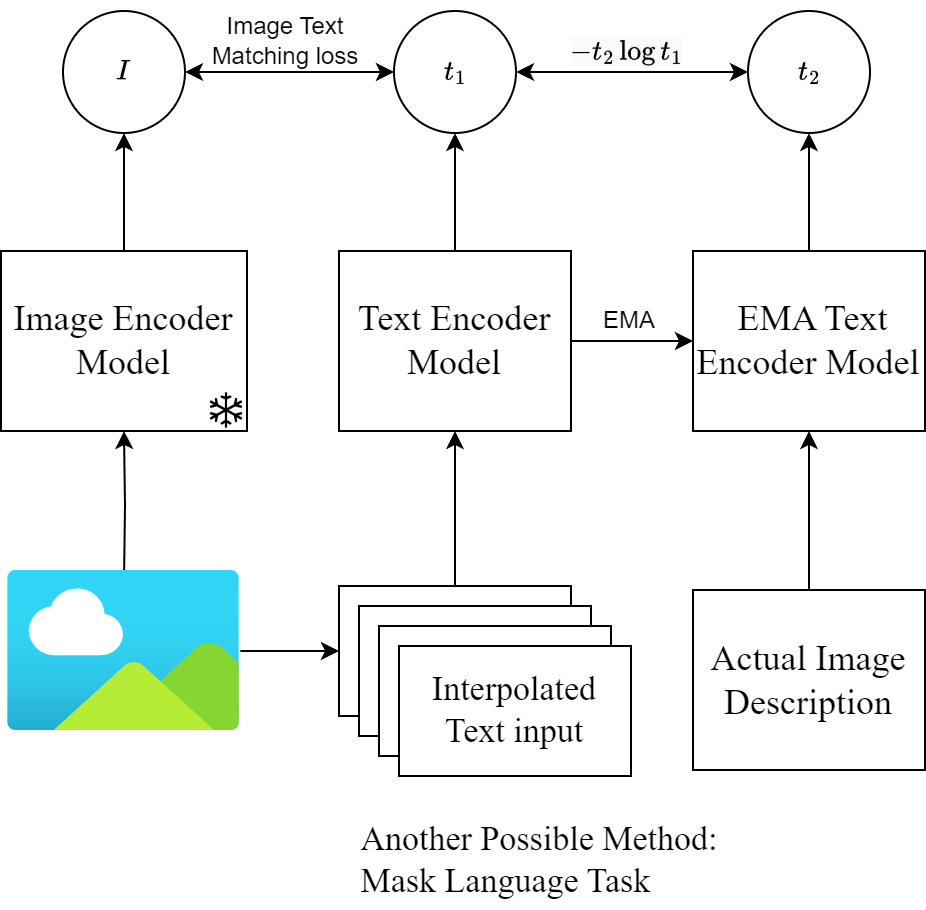
\includegraphics[width=0.8\linewidth]{Images/ThesisDiagram.png}
   \end{center}
   \caption{Overview of proposed method of applying moving average teacher to produce robust text encoder in pre-trained vision language model.}
   \small
\end{figure}


\section{Related work}

\subsection{Vision-Language model}
In the past few years, many works have shown the ability to utilize textual information with the image task by training with image text pair \eg CLIP \cite{clip}, UNITER \cite{uniter}, Blip \cite{blip-1,blip-2}, BEiT \cite{beit-3} and CoCa \cite{coca}.
We can roughly divide the vision language model architecture into two categories.
First, vision and language encoder \eg CLIP, CoCa, ALIGN, and mPlug.
These model focus on maximize alignment of two encoders for vision and language encoding.
By training with a large amount of the image-text pair dataset, the ALIGN model could make up for the noisy image description and surpass the model, which was trained with the benchmark dataset in the zero shot image classification task.
Recently \textbf{Co}ntrastive \textbf{Ca}ptioner (CoCa) \cite{coca} proposed a vision-language encoder-decoder model which was trained with image-text contrastive loss and captioning loss.
Cross attention layers were added to join image-text modality.
% The CoCa model performed linear probing image classification on ImageNet with top-1\% 90.6\% accuracy.
Second methods are single encoder jointly trained with both modalities \eg Uniter \cite{uniter}, BeiT-3 \cite{beit-3}, and VLMO \cite{vlmo}.
These methods concatenated both image and text embedding and utilize multi-head self-attention to joined vision and language modalities.
In this research, we choose to experiment with the vision and language encoders method same as CLIP due to separable encoders for distillation.

\subsection{Knowledge Distillation and Self-Distillation}
Knowledge Distillation was firstly proposed by \cite{knowledge_distill} to compress the model size while maintaining the model performance as much as possible.
The method contained a smaller student model and a single or multiple larger teacher model.
The knowledge was transferred by optimizing the student model output to match the teacher's output.
\cite{born_again} investigated knowledge distillation using a student model size the same as the teacher model, showing improvement in the student model.
Such a method is called self-distillation.
The self-distillation has widely adopted in semi-supervised image classification tasks, such as Mean Teacher \cite{mean_teacher}, EMAN \cite{eman} and FixMatch \cite{fixmatch}.
DINO \cite{dino} proposed self-distillation pre-training without using any label, which resulted in performance improvement.
In this paper, we extended the self-distillation by creating representation which was image-text combined representation, and we trained the student model to match teacher softmax outputs.

\section{Methodology}
In this section we provided our self-distillation method and experiment setup details.
\subsection{Self-Distillation}
   
\subsection{Evaluation}


{\small
\bibliographystyle{ieee_fullname}
\bibliography{references}
}

\end{document}
